
\documentclass[12pt]{cspcccsthesis}
% preamble

\title{Spatiotemporal Localization Model for an AR Navigation System using CNN and LSTM in CSPC}
\authorOne{Gian Carlo B. Bata}
\authorTwo{Jane B. Cagorong}
\authorThree{Aron V. Ibias}
\degree{Bachelor of Science in Computer Science}
\approvaldate{January 1, 2020}
\school{College of Computer Studies}
\adviser{Kaela Marie N. Fortuno, MIT}
\dean{Rosel O. Onesa, MIT}
\committeeMemberOne{Ian P. Benitez, DIT}
\committeeMemberTwo{Rosel O. Onesa, MIT}
\committeeChair{Joseph Jessie S. Oñate, MSc}
\department{}
\thesisAbstract{Lorem ipsum dolor sit amet, consectetur adipiscing elit. Nunc scelerisque hendrerit fringilla. Vestibulum nec nibh nisi. Curabitur iaculis est lorem, vehicula consectetur erat ullamcorper eget. Aliquam cursus mollis pretium. Fusce bibendum ornare nisl quis dictum. Curabitur tincidunt euismod erat, fringilla elementum ex blandit in. Nunc pretium libero non bibendum egestas. Interdum et malesuada fames ac ante ipsum primis in faucibus. Etiam vitae porttitor eros. Suspendisse pretium feugiat dui, sed posuere erat porta eu. Lorem ipsum dolor sit amet, consectetur adipiscing elit. Nunc scelerisque hendrerit fringilla. Vestibulum nec nibh nisi. Curabitur iaculis est lorem, vehicula consectetur erat ullamcorper eget. Aliquam cursus mollis pretium. Fusce bibendum ornare nisl quis dictum. Curabitur tincidunt euismod erat, fringilla elementum ex blandit in. Nunc pretium libero non bibendum egestas. Interdum et malesuada fames ac ante ipsum primis in faucibus. Etiam vitae porttitor eros. Suspendisse pretium feugiat dui, sed posuere erat porta eu}
\keywords{amet, consectetur, adipisci velit}

% document body
\begin{document}

\makeTitlePage{January}{2022}

\begin{frontmatter}
    %
\newacronym{gps}{GPS}{Global Positioning System}
\newacronym{ar}{AR}{Augmented Reality}
\newacronym{ai}{AI}{Artificial Intelligence}
\newacronym{tip}{T.I.P.}{Technological Institute of the Philippines}
\newacronym{dmmmsu}{DMMMSU}{Don Mariano Marcos Memorial State University}
\newacronym{cspc}{CSPC}{Camarines Sur Polytechnic Colleges}
\newacronym{cnn}{CNN}{Convolutional Neural Networks}
\newacronym{lstm}{LSTM}{Long Short-Term Memory}
\newacronym{ml}{ML}{Machine Learning}
\newacronym{cv}{CV}{Computer Vision}
\newacronym{rnn}{RNN}{Recurrent Neural Networks}
\newacronym{svm}{SVM}{Support Vector Machines}

% \makeListOfAcronyms
    
% In \begin{approvalPage}{N}, the parameter N is the number of members in the committee. If this is less than 4, the layout of the page is single-column rather than two-column, so change the value accordingly.

\begin{approvalPage}{3}

% Add people in the following format:
% \committeeMember{Member Name}{Member Department/Position}{Member Affiliation}

\end{approvalPage}
    \makePanelofExaminers{90}
    \makeDedication{Ad Majorem Dei Gloriam}
    
\begin{acknowledgments}

I would like to thank the members of my thesis committee for their help in preparation of this work -- Niles Caulder, without whom I would have been doomed to never complete it, Kimiyo Hoshi, who helped to shed new light on many of my ideas, Pamela Isley, with whom I often disagree but who inspires me to be better, Raymond Palmer, who had no small part to play in the formation of the idea, and Kent Nelson, who always had golden advice.

Special thanks are due to the friends and colleagues who made this work possible. Jimmy Olsen and Pete Ross were invaluable both as friends and as sounding boards for some of my more outlandish ideas. Jack Knight, who I met only briefly, was a major influence, and I'm glad we were able to help each other. 

The author gratefully acknowledges the support for this work offered by S.T.A.R. Laboratories under grant award number 3X29YZ4A, and by the Theodore S. Kord Fellowship. Any views and conclusions contained herein are those of the author, and do not necessarily represent the official positions, express or implied, of the funders.

\end{acknowledgments}

    \makeAbstract
    \makeTOC
    \makeListOfTables
    \makeListOfFigures
\end{frontmatter}

\begin{thesisbody}
    
\chapter{Introduction}
\begin{refsection}

This chapter provides an overview of the study, covering the challenges of campus navigation, its objectives, and its significance. It defines the problem, outlines the goals of the research, and highlights the potential impact of the system. The scope and limitations clarify its boundaries, while the project dictionary and notes provide essential terms and supporting details.

\section{Background of the Problem}

With the rapid advancement of technology, navigation systems have evolved significantly to address these challenges. \gls{gps}, \gls{ar}, and \gls{ai} have played a crucial role in improving navigation by providing real-time location tracking, interactive guidance, and intelligent route optimization \cite{1}. Studies have shown that many students now rely on \gls{gps} and digital maps instead of traditional paper maps for navigation \cite{2}. However, while \gls{gps} is practical for outdoor environments, it lacks precise indoor positioning and does not provide interactive real-time assistance on university campuses \cite{3}.

When navigating an unfamiliar place, many people experience anxiety or hesitation in asking for directions. This challenge is common in university settings, where new students and visitors struggle to locate buildings, offices, and other facilities. In large institutions, complex infrastructure and unclear signage can make navigation even more difficult, especially during peak periods such as exams, when new students often have trouble finding essential offices such as the registrar for enrollment, document requests, or exam-related concerns. Research indicates that first-year students commonly face challenges in navigating campuses due to limited access to buildings and unfamiliarity with the environment. For example, a study highlighted that many first-year students found it difficult to navigate their campus, leading to feelings of disorientation and stress \cite{4}.

Several universities in the Philippines have recognized the importance of improving campus navigation and have developed specialized mobile applications to assist students, faculty, and visitors. For example, the \gls{tip} developed "TIP EXPRESS," an Android-based application that utilizes Google Maps to track the user's current location and plot routes within the Quezon City campus. The app employs a fuzzy logic algorithm to determine the shortest route and a channel selection algorithm to identify nearby users within a specific perimeter, in order to improve navigation efficiency and user experience \cite{5}. Similarly, \gls{dmmmsu} introduced "JUAN: Jerome's Unusual Academy Navigator App," designed to identify users' locations on the South La Union campus without requiring internet connectivity. This app features a bee animation to indicate the user's position, aligning with the university's stinging bees mascot, and was utilized during campus events to familiarize students with important buildings and staff locations \cite{6}.

This issue became evident when the researchers experienced it firsthand during the first week at the \gls{cspc}. The researchers were looking for the Green Building, but to their surprise, all buildings on campus were painted blue. When the researchers asked the campus guards for directions, they pointed at multiple blue buildings, making the researchers even more confused. It was only later that the researchers discovered that the building was called the Green Building, not because of its color but because of its solar panel energy source. This experience highlighted the difficulties of navigating a campus when landmarks and directions are not immediately clear. The researchers had to spend an entire week familiarizing themselves with the locations of various buildings, making it difficult to get to classes on time and reducing overall efficiency. Despite the presence of physical maps and signage, navigation on the \gls{cspc} campus remains a challenge for freshmen, visitors, and even faculty. Many struggle to locate classrooms and offices, especially in the first weeks of the semester, due to unclear building names, inconsistent signage, and difficulty finding the fastest routes between buildings. Traditional navigation methods, such as paper maps and verbal directions, can be outdated or unreliable.

To address these challenges, this study explores the integration of \gls{ar}, \gls{cnn}, and \gls{lstm} networks into a spatiotemporal localization model for campus navigation as a potential solution. \gls{ar} technology can provide interactive real-time visual guides, overlaying step-by-step directions on the user's smartphone screen \cite{7}. \gls{cnn} can help recognize the features of buildings and landmarks, avoiding confusion caused by misleading names or identical building colors \cite{8}. These extracted features are then fed into an \gls{lstm}, which analyzes the sequential spatial data to model how movement influences visual perception. This spatiotemporal approach improves \gls{ar} navigation by improving localization and ensuring a more stable positioning system over time \cite{8}.

Existing campus navigation systems are heavily based on \gls{gps}-based tracking, which lacks indoor precision and does not offer \gls{ai}-driven real-time guidance. Although some universities have digital maps, few have integrated \gls{ar}, \gls{cnn}, and \gls{lstm} into their navigation systems. Furthermore, most navigation applications require a stable internet connection, making them inaccessible to students who cannot afford mobile data or experience connectivity problems on campus. To address this limitation, this study aims to develop a model that can function offline, providing students, faculty, and visitors with a potential solution to navigate the campus without relying on cellular data or Wi-Fi. By integrating \gls{ai} and \gls{ar}, the proposed spatiotemporal localization for the \gls{ar} campus navigation model aims to offer a more intuitive and interactive approach to campus wayfinding. Its offline functionality seeks to make navigation assistance more accessible, especially for students with limited internet access.

\section{Statement of the Problem}

Navigating large campuses such as \gls{cspc} can be challenging, especially for new students and visitors. Many struggle to locate classrooms, offices, and laboratories, wasting time and leading to frustration. This issue is more evident during enrollment, exam periods for admission, and when students need to find essential offices like the registrar.

Current navigation methods, such as printed maps, verbal directions, and \gls{gps} applications, have limitations: maps can be outdated, directions unclear, and \gls{gps} requires an internet connection, which not all students have. In response to these challenges, this study aims to explore the development of an offline \gls{ar} campus navigation model to support a more accessible wayfinding. Specifically, the goal is to develop a spatiotemporal landmark recognition and localization model using \gls{cnn} and \gls{lstm} to help recognize campus buildings and identify the location of the user. Lastly, it intends to assess the effectiveness of the model by analyzing its spatiotemporal localization accuracy. Through this study, it is hoped that the navigation of the campus at \gls{cspc} can be improved, making it easier for students and visitors to find their way.

\section{Objectives of the Study}

The objectives of this study are divided into two categories: general and specific. The general objective defines the overall goal of the study, while the specific objectives break down this goal into measurable and achievable steps. These objectives ensure a structured approach to developing an offline spatiotemporal localization model for an \gls{ar} campus navigation model for \gls{cspc}.

\subsection{General Objective}

This study aims to develop an offline spatiotemporal localization model for an \gls{ar} campus navigation model using \gls{cnn} and \gls{lstm} to provide students and visitors at \gls{cspc} with an interactive and real-time way finding solution.

\subsection{Specific Objectives}

To achieve the general objective, the study sets the following specific objectives.

\begin{enumerate}
    \item Develop a spatiotemporal landmark recognition and localization model using \gls{cnn} and \gls{lstm} networks.
    \item Integrate the developed model for an offline \gls{ar}-based campus navigation prototype for real-time route-finding assistance. 
    \item Evaluate the performance of the model.
\end{enumerate}

\section{Significance of the Study}

The proposed study will be beneficial for the following:

\textit{\textbf{\gls{cspc} Students.}} This model will help \gls{cspc} students navigate the campus efficiently, reducing their anxiety about finding specific buildings. Providing clear directions and interactive guidance helps them adjust to their environment with confidence.

\textit{\textbf{Visitors.}} This would be beneficial to visitors, since this navigation tool will allow them to explore the campus without getting lost, allowing them to quickly find the places they need to go. Creates a positive experience for them, encouraging future visits to the \gls{cspc}.

\textit{\textbf{Guests.}} This application will provide a user-friendly interface for guests attending events or meetings, improving their overall experience and accessibility.

\textit{\textbf{Camarines Sur Polytechnic Colleges.}} This study would benefit \gls{cspc} in improving their campus navigation, which improves their reputation as a smart and welcoming school. It will also help to better manage visitors during events, making everything run more smoothly.

\textit{\textbf{Researchers.}} Current researchers can build on this study to explore new ways to use \gls{ar} and \gls{ml}. The project adds valuable knowledge to the field, helping others create better technologies and solutions.

\textit{\textbf{Future Researchers.}} Future researchers can use the findings of this project to study how \gls{ar} can improve navigation in schools. It opens up new ideas for research and helps inspire new projects in technology.

\section{Scope and Limitation}

This study aims to develop an offline spatiotemporal localization model for an \gls{ar} campus navigation model using \gls{cnn} and \gls{lstm}. The goal is to provide students and visitors to \gls{cspc} with an interactive and real-time way-finding solution that does not require internet connectivity. The project will be conducted over two whole semesters, allowing ample time for development and testing.

However, there are some limitations to this study. One of them is that ARCore, although it supports many devices, does not cover all smartphones, especially older models. Additionally, the model will only be compatible with the Android operating system. Future versions may consider adding support for other platforms to meet the needs of a diverse user base.

\section{Project Dictionary}

To avoid misunderstandings in the terms used, the following are conceptually and operationally defined.

\begin{itemize}

    \item \textbf{Augmented Reality (AR).} \gls{ar} is a technology that overlays digital information onto the real world, enhancing the user's perception of their environment \cite{9}. In this study, \gls{ar} is utilized to provide interactive navigation aids that help users find their way around the campus.
    
    \item \textbf{Artificial Intelligence (AI).} \gls{ai} refers to the simulation of human intelligence processes by machines, particularly computer systems, enabling them to perform tasks that typically require human intelligence, such as visual perception and decision-making \cite{10}. This study employs \gls{ai} to analyze user data and improve navigation accuracy.
    
    \item \textbf{Convolutional Neural Networks (CNN).} \gls{cnn} are a class of deep learning algorithms particularly effective in processing visual data, such as images and videos, by mimicking the way the human brain processes visual information \cite{11}. In this study, \gls{cnn}s are employed to analyze visual inputs from the \gls{ar} system to identify and classify objects on campus.
    
    \item \textbf{\gls{cv}. } \gls{cv} is a field of \gls{ai} that enables computers to interpret and understand visual information from the world, allowing them to make decisions based on that data \cite{12}. This study leverages computer vision to enhance the \gls{ar} navigation experience by recognizing landmarks and providing contextual information.
    
    \item \textbf{Geolocation Systems.} Geolocation systems are technologies that determine the geographic location of a device, often using satellite signals or other data sources \cite{13}. In this study, geolocation systems are essential for providing real-time location tracking and navigation assistance on campus.
    
    \item \textbf{Global Positioning System (GPS).} The \gls{gps} is a satellite-based navigation system that allows a \gls{gps} receiver to determine its exact location (latitude, longitude, and altitude) anywhere on Earth \cite{14}. This study uses \gls{gps} to enable precise location tracking for users navigating the campus.
    
    \item \textbf{Long Short-Term Memory (LSTM).} \gls{lstm} is a type of \gls{rnn} architecture that is capable of learning long-term dependencies in sequential data, making it useful for tasks such as time series prediction and natural language processing \cite{15}. In this study, \gls{lstm} is used to analyze user movement patterns over time, improving the navigation model's responsiveness.
    
    \item \textbf{Landmark Recognition.} Landmark recognition refers to the process of identifying and classifying significant features or objects within a visual scene that aid in navigation and orientation \cite{16}. In the context of this project, landmark recognition specifically involves the navigation model's capability to identify and locate important features or points of interest on the \gls{cspc} campus, such as buildings, signage, and other notable structures.
    
    \item \textbf{Localization Model.} A localization model is a system designed to determine the user's position within a specific environment, employing various sensors and algorithms to provide accurate location data essential for effective navigation \cite{17}. In this project, the localization model will work with the landmark recognition system to enhance the overall way-finding experience for students and visitors at \gls{cspc}.
    
    \item \textbf{Machine Learning.} \gls{ml} is a subset of \gls{ai} that enables systems to learn from data and improve their performance over time without being explicitly programmed \cite{18}. This study incorporates \gls{ml} techniques to refine the navigation algorithms based on user interactions and feedback.
    
    \item \textbf{Navigation Model.} The Navigation Model is a framework that aids users in reaching their destinations by integrating technologies such as \gls{gps} and \gls{ar}, which provide real-time directions and interactive guidance within environments like campuses \cite{19}. In this study, the Navigation Model utilizes \gls{ml} techniques, specifically \gls{cnn} and \gls{lstm} algorithms, to enhance navigation accuracy and adapt based on user interactions and feedback.
    
    \item \textbf{Spatiotemporal}. Spatiotemporal refers to having both spatial and temporal qualities, relating to the interplay of space and time \cite{20}. In this study, spatiotemporal data encompasses information that varies across both locations on campus and times of day, which is crucial for adapting the navigation model to enhance user experience and effectiveness. 
    
\end{itemize}

%=======================================================%
%%%%% Do not delete this part %%%%%%
\clearpage

\printbibliography[heading=subbibintoc, title={\centering Notes}]
\end{refsection}
    
\chapter{Related Literature and Studies}
\begin{refsection}

This chapter provides a comprehensive overview of the literature and studies related to spatiotemporal landmark recognition and localization, focusing on \gls{ar}-based campus navigation. It also synthesizes critical similarities and differences among existing research on \gls{cnn} and \gls{lstm}. Lastly, the chapter identifies a gap in the current literature and discusses how the present study aims to address this gap.

\section{Review of Related Literature and Studies}

\subsection{Spatiotemporal Landmark Recognition and Localization}

Today, modern deep learning techniques are making rapid progress in the field of spatiotemporal landmark recognition and localization. Spatial feature recognition previously required manual labeling, which is quite labor intensive and very inefficient \cite{three}; deep learning, according to recent work, particularly that of \citeauthor{three} \citeyear{three}, has actually improved recognition performance by better elucidation of spatial relationships between objects. 

In addition, \citeauthor{six} \citeyear{six} showcased pre-trained \gls{cnn} models that were effective in extracting spatial features from hyperspectral images for enhanced classification performance, thus establishing the value of transfer learning for improved performance in different image classification tasks bordering on complex geospatial data \cite{six}. The adoption of \gls{ml} in clustering and recognizing spatial data patterns has further widened the horizon of geospatial analysis. \citeauthor{seven} \citeyear{seven} commented that this would help the automatic extraction of considerable patterns from complex datasets, which is very crucial for processing geographical data, such as satellite imagery, and unraveling hidden trends that would aid decision-making \cite{seven}.

In addition, \citeauthor{eight} \citeyear{eight} examined a high-dimensional self-attention mechanism that combines spatial and temporal features to incrementally improve the predictive power behind systematic evaluations with varying neural network architectures. This work stands as an illustration of the growing finesse in the handling of spatiotemporal data \cite{eight}.

The excessive growth of images, especially in web and mobile applications, poses threats to efficient landmark recognition. Traditional methods, such as \gls{svm}, revealed their limitations when handling variations in elevation and structure. Contemporary studies, including \citeauthor{nine} \citeyear{nine}, show that \gls{cnn} architectures such as ResNet-50 have proven successful in achieving high accuracy for the detection of landmarks in various view angles. These advancements justify the abilities of deep learning models, which are helpful in real-world applications, including navigation to identify unlabeled historical landmarks \cite{nine}.

This concludes that the changeover of the spatiotemporal landmark recognition and localization processes into deep learning is reshaping the domain, addressing issues of efficiency and accuracy. Continuous research will positively impact applications in the field with implications that center on advanced capabilities in understanding and articulating spatial environments.

\subsection{\gls{ar}-based Campus Navigation}

Navigating large university campuses can be challenging, especially for new students and visitors unfamiliar with the environment. \gls{ar}-based navigation systems provide an interactive solution, improving indoor and outdoor way-finding by overlaying digital content onto the real world, improving localization accuracy, and offering real-time guidance.  Several studies highlight the practical benefits of \gls{ar} in campus navigation. \citeauthor{one} \citeyear{one} proposed an ARCore-based system that uses visual-inertial ranging and Unity3D to improve positioning in \gls{gps}-limited areas \cite{one}. Similarly, \citeauthor{ten} \citeyear{ten} integrated IoT-based sensor fusion for adaptive route guidance, while \citeauthor{two} \citeyear{two} combined \gls{gps}, Wi-Fi, BLE beacons and \gls{ai}-driven path optimization for voice-assisted, accessible navigation \cite{ten, two}. \citeauthor{thirteens} \citeyear{thirteens} explored \gls{ai} integration through \gls{cnn} and LSTM to improve the precision of localization \cite{thirteens}. Hybrid systems were also developed, such as the \gls{ar}-VR platform by \citeauthor{four} \citeyear{four}, which allows real-time tracking, virtual campus tours and personalized routes, and the landmark-based system by \citeauthor{twelve} \citeyear{twelve}, which improves spatial learning, especially for older adults \cite{four, twelve}.

In addition to supporting indoor-outdoor navigation, \citeauthor{five} \citeyear{five} introduced an \gls{ar} app utilizing computer vision and object detection, while \citeauthor{eleven} \citeyear{eleven} and \citeauthor{fifteen} \citeyear{fifteen} focused on indoor systems that integrate sensor data and \gls{ar} overlays for improved accuracy and user experience \cite{ten, eleven, fifteen}. \citeauthor{fourteen} \citeyear{fourteen} also emphasized the broader developments in \gls{ar}-assisted indoor positioning and mapping technologies \cite{fourteen}.

In conclusion, these studies collectively underscore the potential of \gls{ar}-powered campus navigation systems in delivering accurate, accessible, and interactive guidance. With the integration of real-time tracking, \gls{ai}, and immersive interfaces, \gls{ar} systems continue to enhance the overall wayfinding experience in educational environments.

\subsection{Convolutional Neural Networks}

The integration of \gls{cnn} into \gls{ar}-based navigation systems has significantly enhanced localization accuracy, object recognition, and real-time spatial understanding, making navigation more intelligent and responsive.

Several studies have demonstrated the value of \gls{cnn}s in improving \gls{ar} navigation. \citeauthor{twentytwo} \citeyear{twentytwo} emphasized how \gls{cnn}s enhance scene recognition and real-time interaction in \gls{ar} environments, while \citeauthor{twenty} \citeyear{twenty} developed a \gls{cnn}-augmented SLAM system using planar constraints for more stable positioning \cite{twentytwo, twenty}. Similarly, \citeauthor{seventeen} \citeyear{seventeen} applied \gls{cnn}s to mobile robot localization in indoor spaces, and \citeauthor{twentyfive}\citeyear{twentyfive} extended this by applying deep \gls{cnn}s to dynamic pathfinding in autonomous robot navigation \cite{seventeen, twentyfive}.

Other researchers have focused on \gls{cnn}s to support accessibility. \citeauthor{sixteen} \citeyear{sixteen} implemented \gls{cnn}s in \gls{ar} systems to assist visually impaired users by improving obstacle detection, while \citeauthor{eighteen} \citeyear{eighteen} enhanced environmental perception through \gls{cnn}-powered object recognition and tracking \cite{sixteen, eighteen}. In terms of interaction, \citeauthor{twentyone} \citeyear{twentyone} introduced a \gls{cnn}-based multi-target classification model for \gls{ar}-SSVEP to improve interaction precision \cite{twentyone}.

Broader reviews and advanced implementations further showcase \gls{cnn}'s potential. \citeauthor{nineteen} \citeyear{nineteen} conducted a systematic review of \gls{cnn} use across \gls{ar}, VR, and MR, emphasizing their role in spatial computing and immersive navigation \cite{nineteen}. \citeauthor{twentyfour} \citeyear{twentyfour} combined \gls{cnn}s with LSTM in Kalman filter fusion to refine path correction and trajectory prediction, while Shin-\citeauthor{twentythree} \citeyear{twentythree} demonstrated \gls{cnn}s' value in surgical \gls{ar} navigation requiring high-precision localization \cite{twentyfour, twentythree}.

In conclusion, these studies collectively highlight the critical role of \gls{cnn}s in advancing \gls{ar}-based navigation. By enabling accurate object recognition, adaptive route planning, and robust spatial understanding, \gls{cnn}s contribute significantly to making \gls{ar} navigation systems more intelligent, accessible, and immersive.

\subsection{Long Short-Term Memory}

State-of-the-art positioning technology has traditionally produced large-scale trajectory data that plays a major role in location prediction for location-based services (LBS). Displacement forecast through long-term visitations following the traditional sense or real-time trajectory forecasting are the mainstream methods. An emerging approach has interest in integrating both the spatial and temporal dimensions together using \gls{lstm} Networks, where, even more specifically, the Spatial-Temporal Long Short-Term Memory (ST-LSTM) model tackles data sparsity and caters to better urban mobility and personalized LBS applications \cite{twentysix}. The SPATIAL architecture provides yet another example of such integration with improved prediction accuracy \cite{twentyseven}.

It is noteworthy that Wi-Fi-based positioning has gained some traction, especially in the indoor setting, but with its challenges in accuracy due to varying signal conditions. A recent spatial-temporal positioning algorithm adopts a residual network for the extraction of spatial features and LSTM, greatly increasing the precision of localization \cite{twentyeight}.

LSTMs may also find utilization in environmental monitoring, thus performing weather prediction and applicable scenarios better than traditional \gls{cnn} and LSTM methods with a hybrid model among variates \cite{twentynine}.

Another area is traffic management. According to \citeauthor{thirty} \citeyear{thirty}, LSTM models outperformed classical methods in estimating traffic speed \cite{thirty}. \citeauthor{thirtyone} \citeyear{thirtyone} demonstrated the successful application of the improved Bi-LSTM model to real-time traffic flow forecasting, further stating that spatial-temporal modeling is crucial in urban traffic systems \cite{thirtyone}. \citeauthor{thirtytwo} \citeyear{thirtytwo} improved trajectory prediction of vehicles by using spatial and temporal attention mechanisms in the STAM-LSTM, capable of capturing the relationships between vehicle and associated motion features \cite{thirtytwo}.

Apart from transportation, \gls{lstm} networks have made strides in facial expression recognition; the Enhanced ConvLSTM model leverages the spatial and temporal connections and is efficient in complex environments \cite{thirtythree}. In a parallel manner, the STGA-LSTM framework by \citeauthor{thirtyfour} predicts short-term demand for bike-sharing using Graph Convolutional Networks, witnessing an unprecedented advancement in demand forecasting \cite{thirtyfour}. Then, in predicting outlet temperature for energy systems, a hybrid model \gls{cnn}-LSTM was established on modeling spatial-temporal features for better thermal energy management \cite{thirtyfive}, proposed by \citeauthor{thirtyfive} \citeyear{thirtyfive}.

This coupling of spatial and temporal factors in LSTMs has led to the elimination of boundaries in predictive analytics across various fields. This development indicates that the model may be the answer to stochastic problems posed in real-life scenarios, such as intelligent transportation systems, environmental monitoring, urban mobility, and energy management. LSTM has also begun to set the way for future breakthroughs in predictive modeling and analytics as research continues.

\subsection{Evaluation Metrics and Performance Analysis}

Evaluating the effectiveness of AR-based campus navigation systems requires a comprehensive assessment of their positional accuracy. Different metrics serve to illuminate various aspects of system performance. For large deployable mesh reflectors, \citeauthor{thirtyseven} \citeyear{thirtyseven} highlights the usefulness of the root-mean-square (RMS) error as an effective surface accuracy measure. RMS calculates the average deviation between the actual surface and the intended shape, providing a single value that summarizes overall surface fidelity. Yuan's study compares several RMS measurement approaches: nodal deviation offers highly localized details but demands extensive computational effort; the best-fit surface method provides a balanced, global view of shape accuracy; and direct RMS error yields a simple overall deviation metric, though it may miss localized imperfections. Incorporating assessments focused on critical surface regions enhances the evaluation by highlighting areas most vital to system performance \cite{thirtysix}. 

In the context of indoor positioning, \citeauthor{thirtyseven} \citeyear{thirtyseven} demonstrate the importance of path-based error metrics like the Mean Euclidean Error (MEE). Their research compares different methods and finds that the Visibility Graph (VG) approach achieves the lowest average error of about 2.2 meters, closely reflecting the actual routes pedestrians walk in complex indoor spaces. The Navigation Mesh (NM) method follows with an error near 2.4 meters, while the Fast Marching (FM) method results in a higher average error of approximately 3.7 meters. These findings emphasize that MEE, which measures the length of paths pedestrians would realistically follow, provides a more practical, real-world assessment of localization accuracy than simple straight-line distances. Since MEE closely relates to how users navigate environments, it offers valuable insights into system usability and reliability.  \cite{thirtyseven}. 

The evaluation results for navigation time in the study of \citeauthor{one} \citeyear{one}, indicates that during the experiments, the AR navigation system achieved approximately a 20\% reduction in navigation times compared to traditional maps at Shanghai University, which is a notable improvement in efficiency. The mention of "p < 0.05" refers to the p-value obtained from statistical testing, likely a t-test or similar, which measures the probability that the observed difference occurred by chance. A p-value less than 0.05 is commonly considered statistically significant, meaning there is less than a 5\% probability that the observed reduction in navigation time was due to random variation alone. This significance level provides confidence that the AR system genuinely enhances navigation speed, validating its effectiveness. The combination of practical results (20\% reduction) and statistical validation (p < 0.05) supports the conclusion that the AR-based system offers a meaningful and reliable improvement for campus navigation \cite{one}. 


\section{Synthesis of the State of the Art}

The evolution of spatiotemporal landmark recognition and localization has been significantly shaped by deep learning techniques, particularly with the integration of \gls{cnn} and \gls{lstm} networks. Traditional spatial recognition methods, which relied heavily on manual landmark identification, have proven inefficient and time-consuming \cite{three}. The work of \citeauthor{three} \citeyear{three} emphasized the use of deep learning in enhancing recognition accuracy and spatial relationship modeling \cite{three}. \citeauthor{six} \citeyear{six} highlighted the benefit of transfer learning with pre-trained \gls{cnn}s in improving classification accuracy, especially in hyperspectral imagery \cite{six}. Similarly, \citeauthor{seven} \citeyear{seven} noted that \gls{ml} improved spatial clustering and pattern recognition, which are vital in geospatial analysis \cite{seven}.

To further boost prediction accuracy, \citeauthor{eight} \citeyear{eight} proposed a high-dimensional self-attention mechanism for fusing spatial and temporal features \cite{eight}. In contrast, \citeauthor{nine}\citeyear{nine} pointed out the limitations of traditional algorithms like Support Vector Machines (SVMs), especially when dealing with orientation variations, where \gls{cnn} models such as ResNet-50 performed better in landmark detection \cite{nine}. These advancements have practical applications in navigation, automated mapping, and landmark identification across diverse environments.

\gls{ar}-based campus navigation systems have emerged as practical applications of these models, offering interactive and real-time wayfinding solutions. \citeauthor{one} \citeyear{one} designed an ARCore-based system utilizing visual-inertial ranging algorithms for enhanced positioning, while \citeauthor{ten} \citeyear{ten} incorporated IoT-based sensor fusion to enable adaptive route guidance \cite{one, ten}. Similarly, \citeauthor{two} \citeyear{two} integrated \gls{gps}, Wi-Fi triangulation, BLE beacons, and \gls{ai}-driven path optimization to support voice-assisted and event-based routing \cite{two}. \citeauthor{thirteens} \citeyear{thirteens} focused on \gls{ai}-enhanced \gls{ar} systems using \gls{cnn} and LSTM models to improve navigation accuracy. \citeauthor{four} \citeyear{four} developed a hybrid \gls{ar}-VR system that supports virtual campus exploration and personalized routing \cite{thirteens, four}.

\citeauthor{twelve} \citeyear{twelve} developed a landmark-based navigation system targeting older adults, while \citeauthor{fourteen} \citeyear{fourteen} provided a broad overview of \gls{ar}-assisted localization techniques \cite{twelve, fourteen}. \citeauthor{five} \citeyear{five} emphasized the use of computer vision and object detection, and \citeauthor{eleven} \citeyear{eleven}focused on enhancing indoor navigation through sensor integration \cite{five, eleven}. Lastly, \citeauthor{fifteen} \citeyear{fifteen} streamlined campus wayfinding by overlaying directional markers in \gls{ar} environments. Together, these works highlight the growing impact of \gls{ar} in educational settings for real-time and user-friendly navigation \cite{fifteen}.

\gls{cnn} integration continues to be a major force behind advancements in AR. \citeauthor{twentytwo} \citeyear{twentytwo} and \citeauthor{twenty} \citeyear{twenty} showed how \gls{cnn}s enhance real-time scene recognition and positioning \cite{twentytwo, twenty}. \citeauthor{sixteen} \citeyear{sixteen} and \citeauthor{seventeen} \citeyear{seventeen} applied \gls{cnn}s to assist visually impaired users and optimize indoor navigation \cite{sixteen, seventeen}. \citeauthor{twentyfive} \citeyear{twentyfive}, \citeauthor{eighteen} \citeyear{eighteen}, and \citeauthor{twentyone} \citeyear{twentyone} further validated \gls{cnn}s’ capacity for object recognition and interaction in \gls{ar} contexts \cite{twentyfive, eighteen, twentyone}. \citeauthor{nineteen} \citeyear{nineteen} reviewed \gls{cnn} applications in AR, VR, and MR, while \citeauthor{twentyfour} \citeyear{twentyfour} and \citeauthor{twentythree} \citeyear{twentythree} demonstrated \gls{cnn}s' effectiveness in surgical and predictive navigation systems \cite{nineteen, twentyfour, twentythree}.

\gls{lstm} networks also play an important role by capturing spatial-temporal dependencies in path prediction and localization. \citeauthor{twentysix} \citeyear{twentysix}, \citeauthor{twentyseven} \citeyear{twentyseven}, \citeauthor{twentyeight} \citeyear{twentyeight}, all demonstrated the application of \gls{lstm} networks to improve accuracy in various domains, from location tracking to environmental forecasting \cite{twentysix, twentyseven, twentyeight}. \citeauthor{twentynine} \citeyear{twentynine} and \citeauthor{thirty} \citeyear{thirty} showed \gls{lstm} networks' predictive accuracy in temperature modeling and traffic speed forecasting \cite{twentynine, thirty}. \citeauthor{thirtyone} \citeyear{thirtyone} and \citeauthor{thirtytwo} \citeyear{thirtytwo} focused on \gls{lstm} variants such as Bi-LSTM and STAM-LSTM for vehicle trajectory predictions, while \citeauthor{thirtythree} \citeyear{thirtythree}, \citeauthor{thirtyfour} \citeyear{thirtyfour}, and \citeauthor{thirtyfive} \citeyear{thirtyfive} explored their integration with \gls{cnn} and GCN for specific applications such as emotion recognition and energy modeling \cite{thirtyone, thirtytwo, thirtythree, thirtyfour, thirtyfive}.

In evaluating \gls{ar}-based campus navigation systems, several key metrics are utilized to assess efficiency, accuracy, and reliability. Root Mean Squared Error (RMSE) helps capture significant localization discrepancies by emphasizing larger errors, as supported by \citeauthor{thirtysix} \citeyear{thirtysix}, who demonstrated that RMSE effectively assesses surface accuracy, with methods such as the best-fit surface that offers balanced global evaluations \cite{thirtysix}. Mean Euclidean Error (MEE), according to \citeauthor{thirtyseven} \citeyear{thirtyseven}, provides realistic information on positioning performance by measuring the average distance between predicted and actual paths, and their study shows that VG achieved lower MEE values around ~2.2 meters, highlighting its importance in dynamic real-world environments \cite{thirtyseven}. Navigation time, evaluated in the study by \citeauthor{one} \citeyear{one}, showed that \gls{ar}-based systems reduced navigation time by approximately 20\% compared to traditional map applications, significantly improving user navigation speed and efficiency in campus environments \cite{one}. Together, these metrics; RMSE, MEE, and navigation time offer a comprehensive evaluation of \gls{ar} navigation systems, guiding future improvements to improve precision, operational speed, and overall user experience.

In summary, deep learning and \gls{ar} technologies have converged to significantly improve spatial navigation. \gls{cnn}s and \gls{lstm} networks excel in localization, prediction, and interaction modeling, while the integration of RMSE, MEE, and Navigation Time ensures the continuous advancement of more accurate and user-centric navigation systems.

\section{Gap Bridged by the Study}

Existing studies have shown the success and potential of spatial models for \gls{ar} navigation and positioning. However, there is still room for improvement, especially since many current \gls{ar} navigation systems rely on \gls{gps} which uses internet connectivity and focuses mainly on indoor navigation. This creates a gap in the provision of effective outdoor navigation solutions, particularly in large campus areas where reliable guidance is crucial.

This study aims to address this gap by developing an offline spatiotemporal localization model that uses \gls{cnn} and \gls{lstm} networks. The main goal is to create an interactive way-finding solution for \gls{cspc}.

%=======================================================%
%%%%% Do not delete this part %%%%%%
\clearpage

\printbibliography[heading=subbibintoc, title={\centering Notes}]
\end{refsection}
    
\chapter{Methodology}
\begin{refsection}

This chapter provides the methodology for developing the prototype for the spatiotemporal localization model for an \gls{ar} navigation system in \gls{cspc}, including data collection, pre-processing, \gls{ml} model training and testing, and performance evaluation.

\section{Research Design}

Constructive research design is a strategy for creating new constructs or systems that build on existing knowledge, concepts, or methods to address specific problems or challenges. It involves developing innovative solutions by combining and adapting well\-established theories, techniques, and models to solve real-world problems. This design often relies on a combination of existing tools, knowledge, and frameworks, where researchers adapt and reassemble them into novel constructs or systems. In this process, the research seeks not only to develop theoretical understanding but also to create practical, tangible, functional solutions that can be implemented in real-world settings. This design is particularly relevant in fields where continuous innovation and development are required and where applying existing knowledge to new contexts can lead to breakthroughs in solving emerging problems \cite{crnkovic2010}.

This study will adopt a constructive research design to develop a spatiotemporal localization model for an \gls{ar} navigation system at \gls{cspc}, using \gls{cnn} and \gls{lstm} networks. The constructive research design suits the study well, as it involves combining different existing models and algorithms to create a system that addresses the problem stated in Chapter 1.2. The artifact in this study is a spatiotemporal localization model integrated into a mobile AR navigation application. It is designed to determine user location based on visual cues and sensor data (e.g. rotation vector) collected from the mobile device, without the need for internet connectivity or \gls{gps}. This approach ensures that the \gls{ar} navigation system operates independently of real-time data transmission, making it robust in environments with limited or no network connectivity.

Adopting a constructive research design allows researchers to build on existing methodologies while innovating and developing a new solution that addresses the specific challenges of \gls{ar} navigation in an educational setting. This approach facilitates the creation of an artifact that can function independently of conventional data sources, ensuring that the \gls{ar} navigation system is reliable and effective in dynamic and offline environments. Drawing on existing knowledge and adapting it creatively, the study aims to provide a significant contribution to the field of \gls{ar} navigation and spatiotemporal localization.

\section{Theorems, Algorithms, and Mathematical Models}

In computer science, theorems, algorithms, and mathematical models lay the foundation for \gls{ml} models. This study will use \gls{cnn} together with \gls{lstm} networks for spatiotemporal localization, highlighting their utility in feature extraction and sequential learning for spatiotemporal awareness. In particular, this study will use ResNet-50, which is based on \gls{cnn}, and a regular \gls{lstm} model.

\subsection{ResNet-50 Architecture}

Residual Networks, or ResNets, were introduced to overcome the challenges of training very deep neural networks, particularly the degradation problem, where adding more layers to a network leads to worse performance rather than improved accuracy. Proposed by \citeauthor{he2015deepresiduallearningimage} \citeyear{he2015deepresiduallearningimage}, ResNet introduces the concept of residual learning, where the layers are designed to learn the residual or the difference between the input and the desired output rather than learning the output directly. This is achieved through the use of shortcut connections that skip one or more layers, enabling the network to pass information directly from the earlier to the later layers. These identity shortcuts help preserve gradients during training, effectively mitigating the vanishing gradient problem and making it possible to train networks with hundreds or even thousands of layers \cite{he2015deepresiduallearningimage}.

\begin{figure}[H]
    \centering
	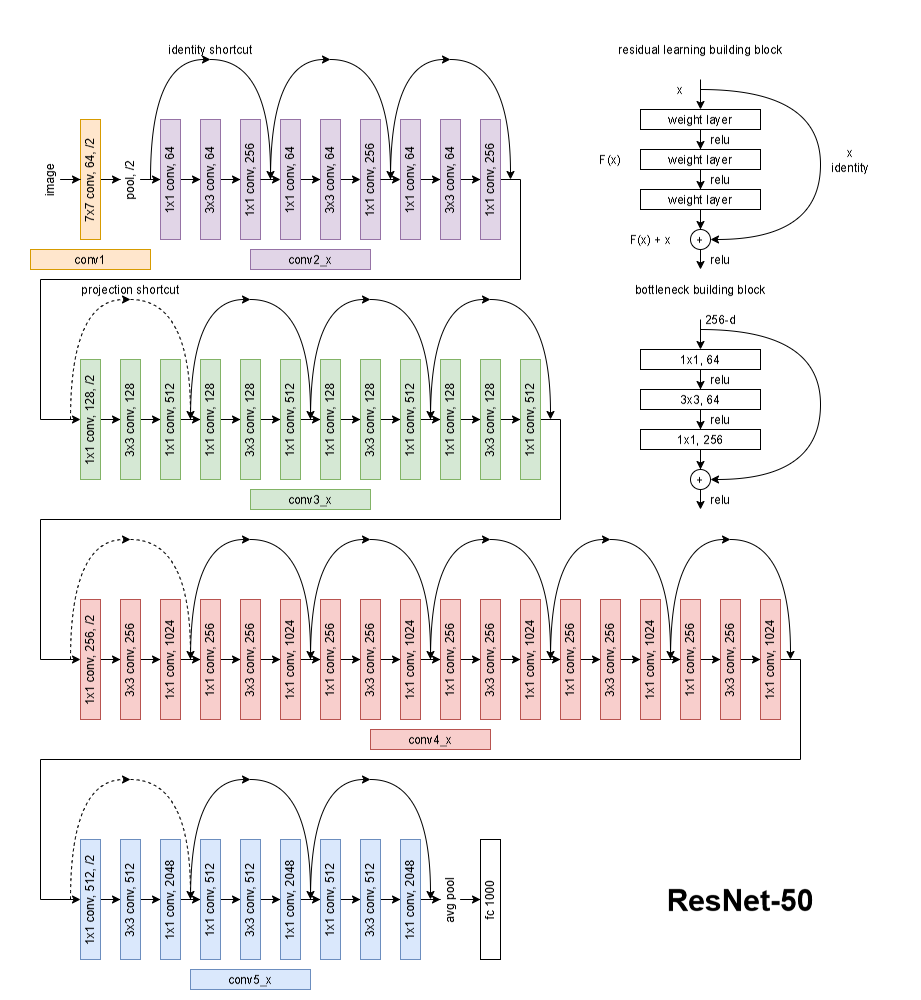
\includegraphics[width=0.85\textwidth]{figures/resnet.png} 
	\caption[ResNet-50 Architecture]{Detailed diagram of the ResNet-50 Architecture.}
	\label{fig:firstFig}
\end{figure}

\ref{fig:firstFig} shows the architecture of ResNet-50, a variant of the Residual Networks architecture consisting of 50 layers, specifically utilizing a bottleneck design that includes three layers per residual block (1x1, 3x3, and 1x1 convolutions). This setup allows for dimension reduction for lighter computation in the later layer and then dimension expansion for the preservation of the block input size. This distinguishes it from shallower versions of ResNet such as ResNet-18 and ResNet-34, which, on the other hand, use two-layer blocks and fewer overall layers, making them less computationally intensive, but also potentially less powerful. In contrast, deeper models such as ResNet-101 and ResNet-152 extend the number of layers and blocks, increasing the capacity at the cost of higher computational complexity. ResNet-50 offers a balance between depth, performance, and computational efficiency, which led the researchers to choose this particular architecture variant. It consist of five residual blocks, namely; conv1, conv2\_x, conv3\_x, conv4\_x, and conv5\_x. Each of these residual blocks output different sizes, which are 112x112, 56x56, 28x28, 14x14, and 7x7 respectively. The final fully-connected later outputs the final 1x1 output size \cite{he2015deepresiduallearningimage}.

For this study, however, the researchers decided to remove the final fully-connected classification layer, as the CNN will be used as a feature extractor instead of its usual use case in classification problems.

\subsection{Main Features of ResNet-50}

\subsubsection{Residual Learning}

ResNet-50 uses residual learning to address the degradation problem in deep networks. Instead of learning the output directly, it learns the residual (the difference between input and output) using shortcut connections. This approach improves the flow of the gradient, allowing training of deeper and more accurate networks.

In the study of \citeauthor{he2015deepresiduallearningimage} \citeyear{he2015deepresiduallearningimage}, the following formulation define the building block of ResNet as:

\begin{equation}
y = F(x, \{W_i\}) + x
\label{eq:bbresnet}
\end{equation}

Where x and y are the respective input and output vectors of the layers considered. The function \(F(x, \{W_i\})\) represents the residual mapping to be learned \cite{he2015deepresiduallearningimage}.

\subsubsection{Identity and Projection Shortcuts}

ResNet-50 uses two types of shortcut connections: identity shortcuts, which directly add input to output when the dimensions match, and projection shortcuts, which use 1x1 convolutions to adjust the dimensions when needed. These shortcuts ensure smooth information flow and support deeper architectures \cite{he2015deepresiduallearningimage}.

\subsubsection{Bottleneck Architecture}

ResNet-50 employs a bottleneck architecture, which consists of three layers: a 1x1 convolution for dimensionality reduction, a 3x3 convolution for feature extraction, and a 1x1 convolution to restore the dimensions. This design reduces computational complexity while maintaining network depth and performance \cite{he2015deepresiduallearningimage}.

\subsection{\gls{lstm} Networks}

Based on the study of \citeauthor{10.1162/neco.1997.9.1.1} \citeyear{10.1162/neco.1997.9.1.1}, \gls{lstm} is a special kind of \gls{rnn} that helps to learn patterns in long sequences of data. Regular \gls{rnn}s have trouble remembering information because they can face issues called vanishing and exploding gradients. \gls{lstm} fixes this by using a special memory cell that can choose what to keep and what to forget.

\ref{fig:secondFig} shows an \gls{lstm} cell's three main parts, called gates: the forget gate, the input gate, and the output gate. These gates control what information to keep or ignore, allowing the network to focus on what is important. This makes \gls{lstm} suitable for tasks such as understanding languages, predicting time series, and analyzing videos \cite{10.1162/neco.1997.9.1.1}.

\begin{figure}[H]
    \centering
	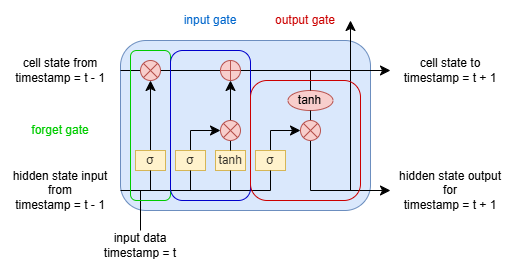
\includegraphics[width=0.85\textwidth]{figures/lstm.png} 
	\caption[An \gls{lstm} Cell]{An \gls{lstm} cell used in \gls{lstm} networks.}
	\label{fig:secondFig}
\end{figure}

\subsection{Core Components of \gls{lstm} Networks}

The core components of \gls{lstm} networks are key to their ability to process sequential data. The cell, or memory, is the central part that stores information over time. The input gate controls what new information gets added to this memory, while the forget gate decides what information should be discarded. Finally, the output gate determines which data will be sent to the next step in the process. Together, these parts help \gls{lstm}s remember important details and learn from sequences, making them great for tasks such as language understanding and time series prediction \cite{10.1162/neco.1997.9.1.1}.

In addition, the following mathematical equations define the gates of \gls{lstm} cells:

\begin{equation}
i_t = \sigma(w_i[h_{t-1}, x_t] + b_i)
\label{eq:igatelstm}
\end{equation}

\begin{equation}
f_t = \sigma(w_f[h_{t-1}, x_t] + b_f)
\label{eq:fgatelstm}
\end{equation}

\begin{equation}
o_t = \sigma(w_o[h_{t-1}, x_t] + b_o)
\label{eq:ogatelstm}
\end{equation}

Where \(i_t\) represents the input gate, \(f_t\) represents the forget gate, \(o_t\) represents the output gate, \(\sigma\) represents the sigmoid function, \(w_x\) is the weight for the respective gate(x) neurons, \(h_{t-1}\) is the output of the previous \gls{lstm} block, \(x_t\) is the input at current timestamp, and \(b_x\) are biases for the respective gates(x).

\section{Material and Evaluation Methods}

The study will use the following materials, tools, and evaluation methods in developing the spatiotemporal localization model.

\subsection{Instruments}

This section contains the dataset, hardware, and software requirements for developing the prototype for the spatiotemporal localization model.

\subsubsection{Dataset}

The study will use a dataset consisting of hyperlapse photographs of the campus and data on sensors and location. These images will be captured at a fixed interval and are sequential, so that the \gls{lstm} networks will have a sensible sequential learning from the data. Along with the images, rotation vector sensor data will be logged whenever an image is captured along with spatial coordinates.

\subsubsection{Hardware}

To support the development and testing of the proposed spatiotemporal localization model for an \gls{ar} navigation system using \gls{cnn} and \gls{lstm}, the researchers will use hardware components that meet or exceed the specifications outlined in Table 1. These components are selected to ensure efficient training of deep learning models and seamless performance of \gls{ar} features in a real-world setting.

\begin{table}[H]
\centering
\caption{Hardware Requirements}
\begin{tabular}{ll}
\hline
\textbf{Component}   & \textbf{Specification}                                                                                      \\ \hline
Processor (CPU)      & Intel i5 (or higher), 2.5 GHz or higher                                                                     \\
Memory (RAM)         & 8 GB (minimum), 16 GB recommended                                                                           \\
Storage              & 500 GB SSD or higher                                                                                        \\
Graphics Card (GPU)  & \begin{tabular}[c]{@{}l@{}}NVIDIA GTX 1060 or higher\\ (for deep learning)\end{tabular}                     \\
Sensors              & \begin{tabular}[c]{@{}l@{}}IMU sensor (Accelerometer,\\ Gyroscope, Magnetometer)\end{tabular}               \\
Mobile Device        & \begin{tabular}[c]{@{}l@{}}Android device with GPS,\\ Accelerometer, Gyroscope,\\ Magnetometer\end{tabular} \\
Camera               & \begin{tabular}[c]{@{}l@{}}High-quality camera\\ (from a Mobile Device)\end{tabular}                        \\
Python               & Version 3.13 or later                                                                                       \\
Jupyter Notebook     & Version 6.0 or later                                                                                        \\
NumPy / Pandas       & Latest version                                                                                              \\
Matplotlib / Seaborn & Latest version                                                                                              \\ \hline
\end{tabular}
\label{tab:firstTab}
\end{table}

To ensure optimal performance of the AR-based campus navigation system, several key hardware components are required. A processor with at least an Intel i5 and 2.5 GHz speed is essential for efficient data processing and model training tasks. Sufficient memory is also crucial; 8 GB of RAM is the minimum, though 16 GB is recommended to handle larger datasets and ensure smoother training operations. For data access and model storage, a 500 GB or larger solid-state drive (SSD) is preferred due to its faster read/write speeds compared to traditional hard drives. Deep learning tasks, especially those involving Convolutional Neural Networks (CNN) and Long Short-Term Memory (LSTM) models, benefit significantly from a dedicated GPU, such as an NVIDIA GTX 1060 or higher, which speeds up training and reduces computation time.

Sensor integration is a vital component of the AR system. An Inertial Measurement Unit (IMU) consisting of an accelerometer, gyroscope, and magnetometer is required to collect movement and orientation data. A compatible Android mobile device equipped with GPS and these sensors is necessary to run the AR interface and capture sensor inputs in real time during navigation. Lastly, a high-quality mobile device camera is used to capture environmental images during data collection. This visual data is essential for landmark detection and localization tasks within the AR system.

\subsubsection{Software}

\begin{table}[H]
\centering
\caption{Software Requirements}
\begin{tabular}{ll}
\hline
\textbf{Component}    & \textbf{Version/Details}        \\ \hline
Android Studio        & Ladybug (2024.2.2) or later     \\
Android SDK           & Latest stable version           \\
Programming Languages & Kotlin                          \\
Pytorch               & Version 2.7 or later            \\
TorchVision           & Compatible with Pytorch version \\
Room Database         & Latest stable version           \\
OpenCV                & Version 4.x or later            \\
Python                & Version 3.13 or later           \\
Jupyter Notebook      & Version 6.0 or later            \\
NumPy / Pandas        & Latest version                  \\
Matplotlib / Seaborn  & Latest version                  \\ \hline
\end{tabular}
\label{tab:secondTab}
\end{table}

\ref{tab:secondTab} shows the software that will be used to develop the underlying technology that will enable the \gls{ar} navigation system in and for \gls{cspc}; listed are the requirements and their respective categories that they fall under.

The development and deployment of the AR-based campus navigation system requires a robust set of software tools and libraries. Android Studio (Ladybug 2024.2.2 or later) serves as the primary integrated development environment (IDE) for building the Android-based AR application. It is supported by the Android SDK, which provides the sensor APIs necessary for access to GPS, accelerometer, and gyroscope. Kotlin is selected as the programming language due to its modern syntax and compatibility with Android development. For deep learning, PyTorch (v2.7 or later) is used to build and train the convolutional neural network (CNN) and long-short-term memory (LSTM) models used in spatio-temporal localization tasks. TorchVision, fully compatible with PyTorch, handles the essential image transformation processes required to train visual models.

To manage and store sensor data collected during user experiments, the Room Database is utilized. It supports structured local data storage within the Android environment. For computer vision tasks such as preprocessing or implementing features like hyperlapse, OpenCV (v4. x or later) is integrated. Python (v3.13 or later) is a core language used for backend model training, preprocessing, and evaluation processes. Additionally, Jupyter Notebook (v6.0 or later) facilitates exploratory data analysis and the visualization of results during development. Lastly, NumPy and Pandas, both at their latest versions, are indispensable for numerical operations and tabular data processing throughout the project.

\subsection{Procedures}

\subsubsection{Data Collection}

The researchers will collect data using hyperlapse recordings, capturing images at regular intervals along predefined paths within the \gls{cspc} campus. Each image will be paired with timestamps, \gls{gps} coordinates, and sensor data. This dataset will be used to train the model to recognize movement patterns and landmarks over time.

\subsubsection{Data Pre-processing}

The collected data will be pre-processed by resizing images and splitting the data into training and validation sets. This will prepare the data for the \gls{cnn}-\gls{lstm} model and ensure that it is ready for training. Specifically, the images will be resized to 224x224 pixels be applied augmentation techniques such as random rotation and brightness adjustments. Sensor data on the other hand will be synchronized with image timestamps using linear interpolation.

\subsubsection{Model Training}

The proposed model is a hybrid architecture that combines \gls{cnn} (ResNet-50) and \gls{lstm} networks. The ResNet-50 component is pretrained on the ImageNet dataset and serves as a feature extractor, producing a fixed-size embedding vector for each image frame. These embeddings are then fed sequentially into a unidirectional \gls{lstm} to learn the temporal dependencies between frames.

During training, the ResNet-50 backbone is initially frozen for the first 10 epochs to allow the LSTM to learn stable temporal patterns. Afterward, the CNN is unfrozen to fine-tune both components jointly. The model is trained for 50 epochs using a batch size of 32 and the Adam optimizer with an initial learning rate of 0.001. Learning rate scheduling and early stop are applied to prevent overfitting. The training objective is to minimize the Mean Squared Error (MSE) between the predicted and actual spatial coordinates.

\subsubsection{Model Testing}

The trained model will be tested on a separate dataset to evaluate its ability to predict locations and track movement under dynamic real-world conditions. Key metrics like accuracy and localization error will be measured. Specifically, by Mean Euclidean Error, Root Mean Squared Error, and Accuracy within a tolerance radius.

\subsubsection{Model Fine-tuning}

The model will be fine-tuned based on testing results. Hyperparameters will be adjusted and specific layers re-trained to improve localization accuracy and robustness under various environmental conditions.

\begin{figure}[H]
    \centering
	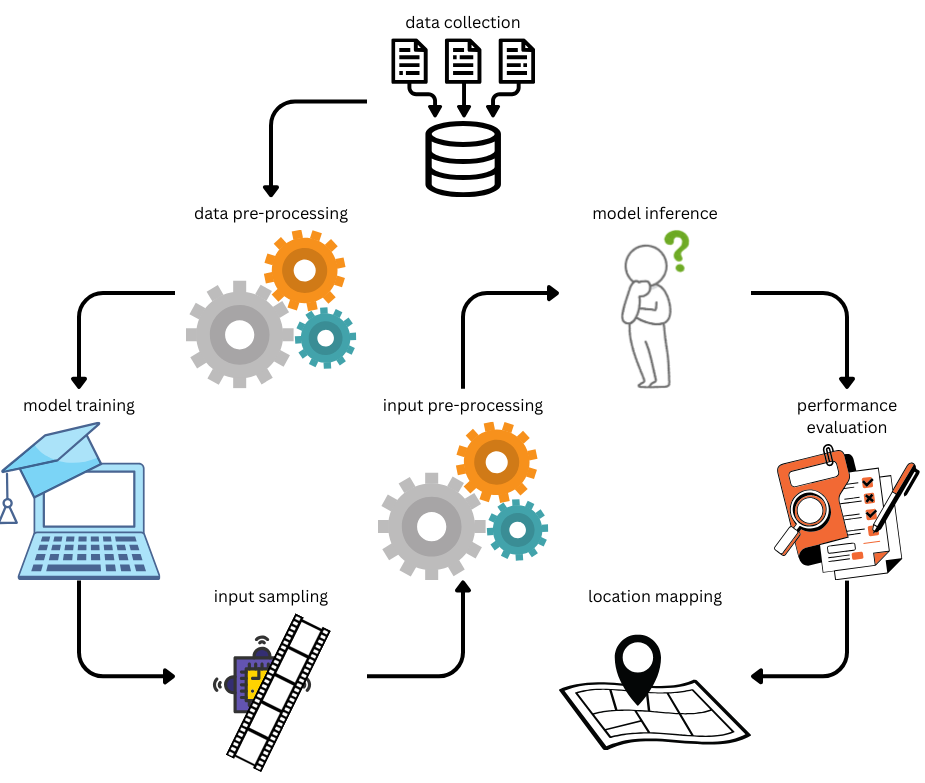
\includegraphics[width=0.7\textwidth]{figures/process.png} 
	\caption[Procedures in the Study]{Flow of the Procedures Used in the Study.}
	\label{fig:thirdFig}
\end{figure}

\subsection{Evaluation Methods}

This section will discuss the evaluation metrics that will be used to measure the performance of the proposed spatiotemporal localization model for an \gls{ar} navigation system. These include the mean Euclidean error, the root mean squared error, the navigation time, and the accuracy of the tolerance radius. These metrics will help determine the effectiveness of the system in recognizing landmarks and assisting users with accurate and efficient \gls{ar}-based navigation.

\subsubsection{Mean Euclidean Error (MEE)}

The Root Mean Squared Error computes the average squared difference between the predicted and actual coordinates. It penalizes larger errors more heavily, making it useful for evaluating sensitivity to outliers. It will be calculated using the following formula:

\begin{equation}
MEE = \frac{1}{n} \sum_{i=1}^{n} \sqrt{(x_i - \hat{x}_i)^2 + (y_i - \hat{y}_i)^2}
\label{eq:mee}
\end{equation}

Where \(n\) is the number of prediction made, \(x_i\) and \(\hat{x}_i\) are the actual and predicted coordinates in the \(x\) axis, while \(y_i\) and \(\hat{y}_i\) are the actual and predicted coordinates in the \(y\) axis. The squaring and rooting in the formula makes it so that computed value will equate to a Euclidean distance.

This metric will provide a human-friendly view of the model's correctness in identifying spatiotemporal landmarks \cite{gmd-15-5481-2022}.

\subsubsection{Root Mean Squared Error (RMSE)}

The Root Mean Squared Error computes the average squared difference between the predicted and actual coordinates. It penalizes larger errors more heavily, making it useful for evaluating sensitivity to outliers. It will be calculated using the following formula:

\begin{equation}
RMSE = \sqrt{\frac{1}{n} \sum_{i=1}^{n} [(x_i - \hat{x_i})^2 + (y_i - \hat{y_i})^2]}
\label{eq:rmse}
\end{equation}

Where \(n\) is the number of prediction made, \(x_i\) and \(\hat{x}_i\) are the actual and predicted coordinates in the \(x\) axis, while \(y_i\) and \(\hat{y}_i\) are the actual and predicted coordinates in the \(y\) axis.

This metric will help analyze the variance of the model and detect large deviations in prediction \cite{gmd-15-5481-2022}.

\subsubsection{Navigation Time}

Navigation time will measure how long it takes users to reach their destinations using the system. Although it does not use a traditional formula, it will be recorded in seconds and used to evaluate the performance and efficiency of the system in real time to guide users through the campus \cite{one}.

\subsubsection{Rate of Prediction Within a Tolerance Radius}

The rate of predictions within a tolerance radius will quantify the frequency with which the model makes predictions within a tolerance radius of the actual coordinates. It will be calculated using the following equation:

\begin{equation}
A_{r \leq x} = \frac{countof\{r_i \mid r_i \leq x\}}{n} \times 100\%
\label{eq:acc}
\end{equation}

Where \(A\) is the accuracy where \(r \leq x\), \(r\) are the predicted radii, \(x\) is the tolerance radius, \(countof\{r_i \mid r_i \leq x\}\) represents the cardinality of the set where \(r_i \leq x\) holds true, including duplicates, \(n\) represents the count of all samples, and the multiplication with \(100\%\) makes the fraction more readable for humans.

This metric will provide information on how frequently the model makes a prediction that is within a tolerance radius.

\section{Conceptual Framework}

The conceptual framework for this study is designed to guide the development of a spatiotemporal localization model for an \gls{ar} navigation system using \gls{cnn} and \gls{lstm} networks at \gls{cspc}. The framework explores the relationships between sensor data, visual input, the deep learning models used for feature extraction and sequence prediction, and the output of the \gls{ar} navigation system.

\subsection{Independent Variables (IVs)}

The independent variables for this research are sensor data and visual data. Sensor data plays a crucial role in providing real-time measurements of the user's orientation, position, and movement within the physical environment. This data includes readings from various sensors such as the accelerometer, gyroscope, magnetometer, and rotation vector sensors, which are typically employed in mobile devices to capture the user's motion and orientation.
Visual data, which includes images or video frames captured by a camera, serves as another key independent variable. The images are used to aid the system's understanding of the user's surroundings, providing contextual information to improve navigation accuracy.

\subsection{Mediating Variables}

The study integrates deep learning models as mediating processes between the raw input data and the final localization output. The first step involves feature extraction using \gls{cnn}. \gls{cnn}s are employed to analyze visual data and extract relevant spatial features from the environment, such as key points or landmarks, that aid in localization. These features are critical in understanding the static and dynamic aspects of the environment, allowing for more accurate mapping.
The second key mediating process involves the use of \gls{lstm} networks, a type of \gls{rnn} designed to handle temporal data. \gls{lstm}s are particularly suited for sequence modeling, enabling the system to learn the temporal dependencies of sensor data over time. By incorporating both past and present data, \gls{lstm}s help predict the user's position and trajectory based on their movement history and environmental context.

\subsection{Dependent Variable (DV)}

The dependent variable in this framework is the localization output, which refers to the predicted position or coordinates of the user within the \gls{ar} navigation system. The goal is to estimate the user's real-time location accurately and in a spatiotemporal context, allowing the \gls{ar} system to display relevant information at the correct location in the physical world.

\subsection{Moderating Variables}

The environmental conditions, such as the layout of the environment (e.g., indoor vs. outdoor spaces) and lighting conditions, may act as moderating variables. These factors influence the effectiveness of both the sensor data and the \gls{cnn}-\gls{lstm} model's performance. For instance, in low-light conditions, the accuracy of visual data may decrease, impacting the feature extraction process. Similarly, complex or cluttered environments may present challenges in accurately predicting the user's location due to increased noise in the sensor readings.

\begin{figure}[H]
    \centering
	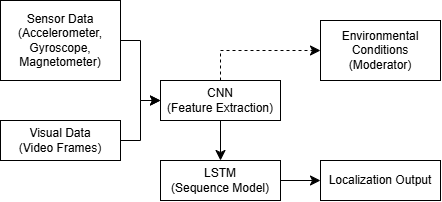
\includegraphics[width=0.85\textwidth]{figures/framework.png} 
	\caption[Conceptural Framework]{Conceptual Framework of the Study.}
	\label{fig:forthFig}
\end{figure}

\subsection{Diagram of Conceptual Framework}

The conceptual framework can be visually represented in \ref{fig:fourthFig} where the independent variables (sensor and visual data) are processed through \gls{cnn} and \gls{lstm} models, with the final outcome being the estimated localization output. Environmental conditions moderate the relationship between the inputs (sensor data and visual data) and the model's ability to predict accurate location estimates.

%=======================================================%
%%%%% Do not delete this part %%%%%%
\clearpage

\printbibliography[heading=subbibintoc, title={\centering Notes}]
\end{refsection}
    
\chapter{Results and Discussion}
\begin{refsection}



%=======================================================%
%%%%% Do not delete this part %%%%%%
\clearpage

\printbibliography[heading=subbibintoc, title={\centering Notes}]
\end{refsection}
    
\chapter{Conclusion}
\begin{refsection}



%=======================================================%
%%%%% Do not delete this part %%%%%%
\clearpage

\printbibliography[heading=subbibintoc, title={\centering Notes}]
\end{refsection}
    \makeBibliography
    
% The environment used here (theappendices) is a wrapper for the basic appendices environment which changes the appearance of the title page and the structure and appearance of the appendices in the table of contents and PDF bookmarks. The original functionality can be restored by simply removing the 'the' from the \begin{} and \end{} statements below.

\begin{theappendices}

\chapter{Language Editing Certification}
\centering

This is to certify that the undersigned has reviewed and went through all the pages of the Bachelor of Science in Computer Science thesis manuscript titled \\

\textbf{"ENTER YOUR TITLE HERE"} \\


of \textbf{AuthorName1}, \textbf{AuthorName2}, \textbf{AuthorName3}, as against the set of structural rules that govern research writing in accord with the composition of sentences, phrases, and words in the English language.
 \newline \newline \newline \\

\noindent \textbf{JUAN DE LA CRUZ} \\
\textit{Language Editor} \\

Date:\_\_\_\_\_\_\_\_\_\_\_\_\_\_\_\_\_\_\_\_\_\_\_


\chapter{Secretary's Certification}
\centering

This is to certify that the undersigned has provided accurate recommendations, suggestions, and comments unanimously agreed and approved by the panel of examiners during the oral examination of the thesis titled \\ \textbf{"ENTER YOUR TITLE HERE"} \\  prepared and submitted by \textbf{AuthorName1}, \textbf{AuthorName2}, \textbf{AuthorName3}, and that the same have not been amended, modified or obliterated. \newline \newline \newline \\



\textbf{MS. MARIA DAISY R. BELARDO} \\
\textit{Secretary} \\


Date:\_\_\_\_\_\_\_\_\_\_\_\_\_\_\_\_\_\_\_\_\_\_\_

\chapter{JOINT AFFIDAVIT OF UNDERTAKING (Plagiarism)}

\centering

\textbf{JOINT AFFIDAVIT OF UNDERTAKING}


% IN WITNESS WHEREOF, I have hereunto set my name this ____ day of ___________ 202__ in
% ___________________________________, Philippines.
% SUBSCRIBED AND SWORN TO before me this ___ day of ________ at _______________, Philippines,
% affiants exhibiting to me their competent proofs of identity above stated.
% Doc. No. ___________:
% Page No.: __________:
% Book No.: __________:
% Series of 202_.


\end{theappendices}
    % Vita should only be included for PhD candidates.

\begin{vita}

\begin{itemize}
    \item 
    
    \begin{figure}[ht]
        \centering
    	
\includegraphics[width=0.35\textwidth]{figures/person-icon.png}
    \end{figure}
    
    \textbf{Joseph Jessie S. Oñate} is a faculty member of the College of Computer Studies. He finished his Master of Science in Computer Science degree at Ateneo de Naga University. His research interests focused on Intelligent Systems, Algorithm and Complexity, Web Technologies, Computer Vision, and Graphics.
    
    \item 
    
    \begin{figure}[ht]
        \centering
    	
\includegraphics[width=0.35\textwidth]{figures/person-icon.png}
    \end{figure}
    
    \textbf{Joseph Jessie S. Oñate} is a faculty member of the College of Computer Studies. He finished his Master of Science in Computer Science degree at Ateneo de Naga University. His research interests focused on Intelligent Systems, Algorithm and Complexity, Web Technologies, Computer Vision, and Graphics.
    
    \item 
    
    \begin{figure}[ht]
        \centering
    	
\includegraphics[width=0.35\textwidth]{figures/person-icon.png}
    \end{figure}
    
    \textbf{Joseph Jessie S. Oñate} is a faculty member of the College of Computer Studies. He finished his Master of Science in Computer Science degree at Ateneo de Naga University. His research interests focused on Intelligent Systems, Algorithm and Complexity, Web Technologies, Computer Vision, and Graphics.
\end{itemize}

\end{vita}
\end{thesisbody}

\end{document}
